\documentclass{article}
\usepackage{graphicx} % Required for inserting images

\title{\textbf{ELL715}\\
\textsc{Project Report (Group 9)} \\ Vessel Enhancement}

\author{
Aditya Singh (2020EE10461) \\
Ananya M (2020MT10787)\\
Harsh Swaika (2021EE11052)\\
Sarthak Srivastava (2020EE10550)\\
Pramod Prasad (2022BSZ8403)
}
\date{November 2023}

\begin{document}

\maketitle

\section{Problem Statement}
We are given retinal scanned images. We have to enhance the blood vessels present in the images of the eye, using image processing

\subsection{Dataset}
We use DRIVE dataset.
It has two folders, \texttt{test} and \texttt{training}. Each folder contains sub-folders named \texttt{images}, \texttt{1st\_manual}, \texttt{masks}.
\begin{enumerate}
    \item \texttt{images} contains 20 fundus images which are considered input in all problems.
    \item  \texttt{1st\_manual} contains the labelled fundus images corresponding to the original ’images’, known as ground truths, which are the expected output of retinal vessel segmentation
    \item  \texttt{masks} are used to define the region of interest (ROI) and can be multiplied to the retinal images at any stage to get rid of unnecessary pixels.
\end{enumerate}

\subsection{Past Work}
We find Sidra Aleem et Al's paper \texttt{Fast and Accurate Retinal Identification System: Using Retinal Blood Vasculature Landmarks}[2019] useful for our project. It discusses processing and matching of retinal images for a retinal identification system with Identification and Enrollment modules.

% https://ieeexplore.ieee.org/abstract/document/8536397
\clearpage
\section{Method}
We will approach the problem by first preprocessing the images, then enhancing using filters, and finally post-processing and evaluating the result.
\subsection{Pre-Processing}
\subsubsection{Green Channel Extraction}
We first pick the green channel from the image to get a better contrast as the retinal vessels are most visible in green channel. Green channel gives best separability of the vessels from the eye fluid

\subsubsection{CLAHE Histogram Equalization}
Contrast Limited Adaptive Histogram Equalization performs histogram equalization in small patches or small tiles with high accuracy and contrast limiting. The neighboring tiles are then combined using bilinear interpolation to remove the artificial boundaries. CLAHE limits contrast amplification to reduce noise amplification

\subsubsection{OTSU Thresholding}
We use OTSU threshold to find the boundary mask to remove small noise from black background. OTSU finds the globally optimal thresholding value then applies it to the image, giving best separation of 2 parts.
The algorithm exhaustively searches for the threshold that minimizes the intra-class variance, defined as a weighted sum of variances of the two classes:

$\sigma _{w}^{2}(t)=\omega _{0}(t)\sigma _{0}^{2}(t)+\omega _{1}(t)\sigma _{1}^{2}(t)$
\subsubsection{Morphological Transform}
Image Opening (Erosion Followed by Dilution) opens the white area and closes the black vessels
\subsubsection{Boundary Removal}
To remove the outer circle from image, we take the circular disk mask then erode it with a \textbf{circular kernel}. Then mask the image with this eroded mask.

$\beta(A) = A - A \ominus B$

\clearpage

\subsection{Vessel Enhancement}
We use \textbf{Frangi filter} to enhance the image.
Frangi filter measures how elongated an image region is, so it detects vessels as objects that are \textit{"long"} and not \textit{"blobby"}


\subsection{Post-Processing}

\subsubsection{Multilevel OTSU Thresholding}
In this multiple threshold levels are selected on histogram and group the pixels of an image into different regions to 
maximize the inter-class variance.

\subsubsection{Wavelet-Based Segmentation}
We use \textbf{bior1.3} wavelets to segment the image further.

\subsubsection{K-means Segmentation}
Used to segment the interest area from the background. It clusters, or partitions the given data into K-clusters or parts based on the K-centroids. K=2 was chosen.


\section{Results}
We run the process on 20 images from the dataset, and report the results by checking if the pixels are matching or not in the output and the ground truth. We count the pixels and report in this table.
\subsection{Sample Outputs}
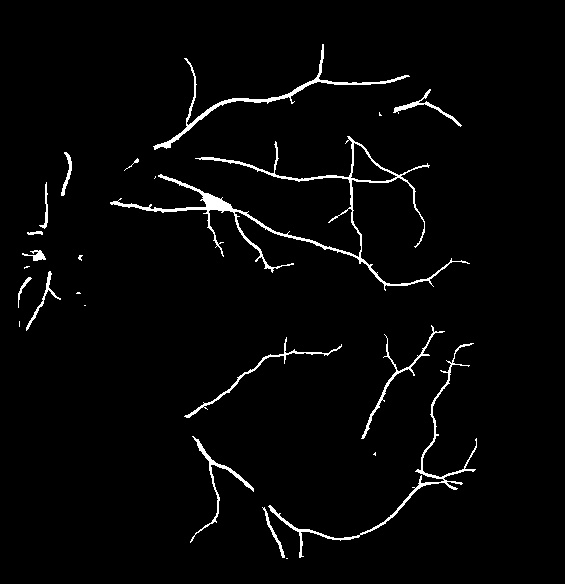
\includegraphics[width=0.3\textwidth]{results/final_21.jpg}
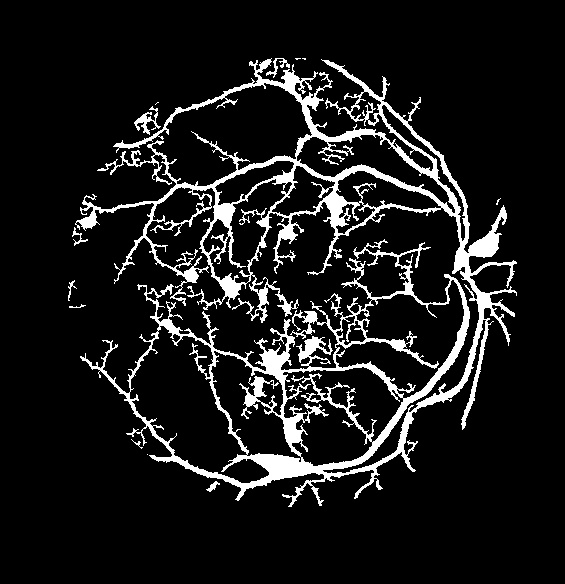
\includegraphics[width=0.3\textwidth]{results/final_25.jpg}
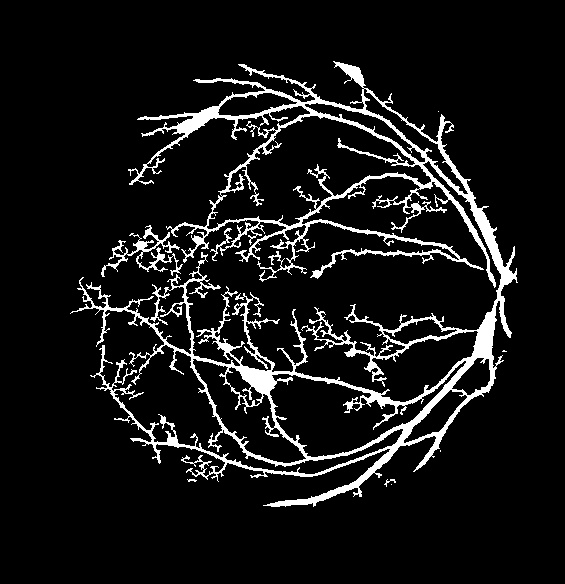
\includegraphics[width=0.3\textwidth]{results/final_30.jpg}
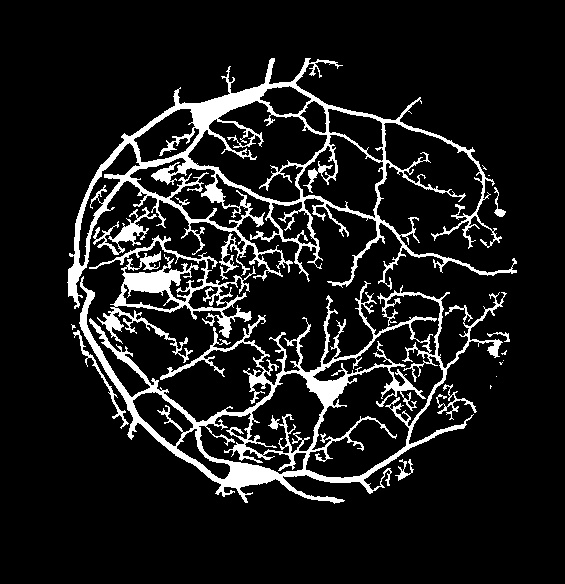
\includegraphics[width=0.3\textwidth]{results/final_35.jpg}

\subsection{Numerical Analysis}
\begin{center}
    \begin{tabular}{|l|l|l|l|l|l|l|l|}
    \hline
        Image & True & True & False & False & Accuracy & Sensitivity & Specificity \\
        \# & Positive & Negative & Positive & Negative & (\%) &  (\%) & (\%) \\ \hline
        1 & 8857 & 295044 & 10258 & 15801 & 92.10 & 46.34 & 94.92 \\ \hline
        2 & 9954 & 290684 & 9467 & 19855 & 91.11 & 51.25 & 93.61 \\ \hline
        3 & 6940 & 287263 & 20974 & 14783 & 89.16 & 24.86 & 95.11 \\ \hline
        4 & 13602 & 281947 & 9784 & 24627 & 89.57 & 58.16 & 91.97 \\ \hline
        5 & 8926 & 292148 & 6143 & 22743 & 91.25 & 59.23 & 92.78 \\ \hline
        6 & 9731 & 292734 & 9653 & 17842 & 91.67 & 50.20 & 94.26 \\ \hline
        7 & 8886 & 289800 & 11087 & 20187 & 90.52 & 44.49 & 93.49 \\ \hline
        8 & 11065 & 286202 & 11530 & 21163 & 90.09 & 48.97 & 93.11 \\ \hline
        9 & 9586 & 292738 & 9471 & 18165 & 91.62 & 50.30 & 94.16 \\ \hline
        10 & 7004 & 294056 & 10020 & 18880 & 91.24 & 41.14 & 93.97 \\ \hline
        11 & 6042 & 300307 & 9755 & 13856 & 92.84 & 38.25 & 95.59 \\ \hline
        12 & 8706 & 292874 & 10102 & 18278 & 91.40 & 46.29 & 94.13 \\ \hline
        13 & 9233 & 293144 & 10130 & 17453 & 91.64 & 47.68 & 94.38 \\ \hline
        14 & 11065 & 286202 & 11530 & 21163 & 90.09 & 48.97 & 93.11 \\ \hline
        15 & 10076 & 288652 & 12696 & 18536 & 90.53 & 44.25 & 93.97 \\ \hline
        16 & 11519 & 282927 & 11149 & 24365 & 89.24 & 50.82 & 92.07 \\ \hline
        17 & 9876 & 288298 & 12821 & 18965 & 90.37 & 43.51 & 93.83 \\ \hline
        18 & 9431 & 289128 & 12355 & 19046 & 90.48 & 43.29 & 93.82 \\ \hline
        19 & 9608 & 289236 & 12376 & 18740 & 90.57 & 43.70 & 93.92 \\ \hline
        20 & 8179 & 292780 & 12179 & 16822 & 91.21 & 40.18 & 94.57 \\ \hline
        \multicolumn{5}{|c|}{\textbf{Average}}  & \textbf{90.84} & \textbf{46.09} & \textbf{93.84} \\ \hline
        \multicolumn{5}{|c|}{\textbf{Standard Deviation}} & \textbf{0.95} & \textbf{7.32} & \textbf{0.92} \\ \hline
    \end{tabular}
\end{center}


The final Average accuracy is \textbf{90.84\%}, sensitivity is \textbf{46.09\%} and specificity is \textbf{93.84\%}

\section{Code and Images}
We have attached the code as \texttt{code.ipynb} file and the output images as \texttt{results/} along with this report.

\end{document}
